\documentclass{beamer}
\usepackage{caption}
\usepackage{float}
\usepackage{lscape}
\usepackage{graphicx}% http://ctan.org/pkg/graphicx
\usepackage{booktabs}% http://ctan.org/pkg/booktabs
\usepackage{array}
\usepackage[export]{adjustbox}
\usepackage{amsmath}
\usepackage{amsfonts}
\usepackage{amssymb}
\usepackage{tikz}
\usepackage{ upgreek }
\usepackage{subcaption}
\usepackage{tabularx} 
\usepackage{setspace}



\graphicspath{ {images/} }
\usetheme{Madrid}
\definecolor{Gold}{RGB}{218,165,32}
\setbeamertemplate{navigation symbols}{}
\setbeamertemplate{theorems}[numbered]
\setbeamertemplate{theorems}[ams style] 
\renewcommand{\qedsymbol}{$\blacksquare$}

\makeatletter

\setbeamerfont{footline}{size=\fontsize{6}{8.5}\selectfont}

\defbeamertemplate*{footline}{Dan P theme}
{
  \leavevmode%
  \hbox{%
  \begin{beamercolorbox}[wd=.14\paperwidth,ht=2.25ex,dp=1ex,center]{author in head/foot}%
    \usebeamerfont{author in head/foot}\insertshortauthor\expandafter\beamer@ifempty\expandafter{\beamer@shortinstitute}{}{~~(\insertshortinstitute)}
  \end{beamercolorbox}%
  \begin{beamercolorbox}[wd=.63\paperwidth,ht=2.25ex,dp=1ex,center]{title in head/foot}%
    \usebeamerfont{title in head/foot}\insertshorttitle
  \end{beamercolorbox}%
  \begin{beamercolorbox}[wd=.23\paperwidth,ht=2.25ex,dp=1ex,right]{date in head/foot}%
    \usebeamerfont{date in head/foot}\insertshortdate{}\hspace*{1.5em}
\insertframenumber{} / \inserttotalframenumber\hspace*{4ex} 
  \end{beamercolorbox}}%
  \vskip0pt%
}
\makeatother

\title{Cross-Industry Dispersion and the Cross-Section of Expected Returns \\ (Pinchuk 2019)}

% A subtitle is optional and this may be deleted
%\subtitle{Optional Subtitle}

\author{Mykola Pinchuk}

\date{11/05/2019}

\subject{Empirical Asset Pricing}

\AtBeginSubsection[]

\begin{document}

\begin{frame}
  \titlepage
\end{frame}



\begin{frame}{Introduction}
\begin{itemize}
    \item {The economy has permanently evolving structure.}
    \item {Accelerated rate of sectoral transformation creates unemployment risk for workers in declining industries.}
    \item {Many workers posses significant industry-specific skills.}
    \item {Sectoral shifts create labor income risk for workers with industry-specific skills.}
    \item {Since employees can not fully hedge labor risk, it should be relevant for asset pricing.}
    \item {Is the rate of sectoral shifts a state variable?}
\end{itemize}

\end{frame}


\begin{frame}{Key results}
\begin{itemize}
    \item {I use cross-industry dispersion (CID) to measure the rate of sectoral shifts.}
    \item {CID is cross-sectional standard deviation of the returns of industry portfolios.}
    \item {Stocks with high sensitivity to CID produce low returns.}
    \item {This return spread is not explained by common factors.}
    \item {Unlike CID, within-industry dispersion (WID) is not priced.}
    \item {Consistent with the hypothesis that CID proxies for labor risk from sectoral shifts, it predicts unemployment.}
\end{itemize}
\end{frame}



\begin{frame}{Literature}{Related asset pricing literature on idiosyncratic risk}
\begin{itemize}
    \item {Theory:}
    \begin{itemize}
        \item {Constantinides and Duffie (1996). Heterogeneous-agent model, where cross-sectional variance of income growth is a state variable.}
    \end{itemize}
    \item {Empirical papers on idiosyncratic risk:}
    \begin{itemize}
        \item {Ang, Hodrick, Xing and Zhang (2006): High sensitivity to VIX is related to low returns.}
        \item {Herskovic, Kelly, Lustig and Van Nieuwerburgh (2016): High sensitivity to common idiosyncratic volatility (CIV) is related to low returns.}
        \item {Verousis and Voukelatos (2018): High sensitivty to cross-sectional dispersion (CSD) is related to low returns.}
    \end{itemize}
\end{itemize}
\end{frame}



\begin{frame}{Literature}{Macroeconomic literature on unemployment and sectoral shifts}
\begin{itemize}
    \item {Lilien (1982): Unemployment is driven by two forces: aggregate shocks and sectoral shifts. Most of employment fluctuations in 1970s were driven by sectoral reallocation shocks.}
    \item {Loungani, Rush and Tave (1990): Sectoral shifts, proxied by the index of stock market dispersion, predict unemployment at annual frequency.}
    \item {Brainard and Cutler (1993): Sectoral reallocation shocks account for a large fraction of varition in long-term unemployment.}
\end{itemize}
\end{frame}



\begin{frame}{Relationship to literature}
\begin{itemize}
    \item {Bridges the gap between macro and asset pricing literature.}
    \item {Shows asset pricing implications of unemployment, driven by sectoral shifts.}
    \item {Provides evidence, broadly consistent with the model of Constantinides and Duffie (1996).}
    \item {Provides fundamental economic explanation for the cross-sectional returns predictability by CSD (Verousis and Voukelatos 2018). This predictability is driven by cross-industry component of CSD (i.e., CID).}
\end{itemize}
\end{frame}



\begin{frame}{Data}
\end{frame}



\begin{frame}{Cross-Industry Dispersion}

\begin{table}[!htbp] \centering 
  \caption*{\textbf{Table 1: Correlations of changes in CID with changes in other variables}} 
  \label{} 
\scriptsize
\vspace{-0.1cm}
\begin{tabular}{@{\extracolsep{5pt}} ccccccc} 
\\[-1.8ex]\hline 
\hline \\[-1.8ex] 
 & VIX & FU & MU & VOL & CIV & CID \\ 
\hline \\[-1.8ex] 
VIX & $1$ & $0.40$ & $0.36$ & $0.34$ & $0.50$ & $0.11$ \\ 
FU & $0.40$ & $1$ & $0.44$ & $0.30$ & $0.39$ & $0.18$ \\ 
MU & $0.36$ & $0.44$ & $1$ & $0.11$ & $0.24$ & $0.06$ \\ 
VOL & $0.34$ & $0.30$ & $0.11$ & $1$ & $0.27$ & $0.27$ \\ 
CIV & $0.50$ & $0.39$ & $0.24$ & $0.27$ & $1$ & $0.22$ \\ 
CID & $0.11$ & $0.18$ & $0.06$ & $0.27$ & $0.22$ & $1$ \\ 
\hline \\[-1.8ex] 
\end{tabular} 
\end{table}
\end{frame}



\begin{frame}{Time series of CID}
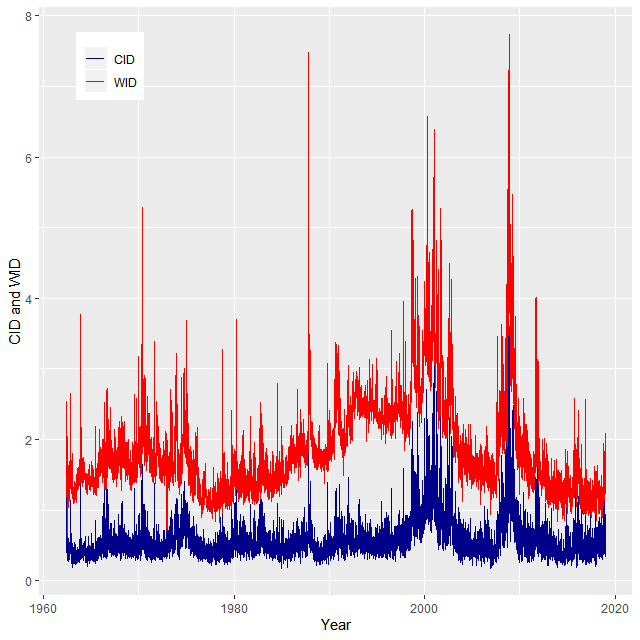
\includegraphics[width=0.64\textwidth]{paper_b3/Figure1.png}
\end{frame}



\begin{frame}{Estimation of $\beta_{CID}$}
\end{frame}



\begin{frame}{Pre-ranking and post-ranking $\beta_{CID}$}
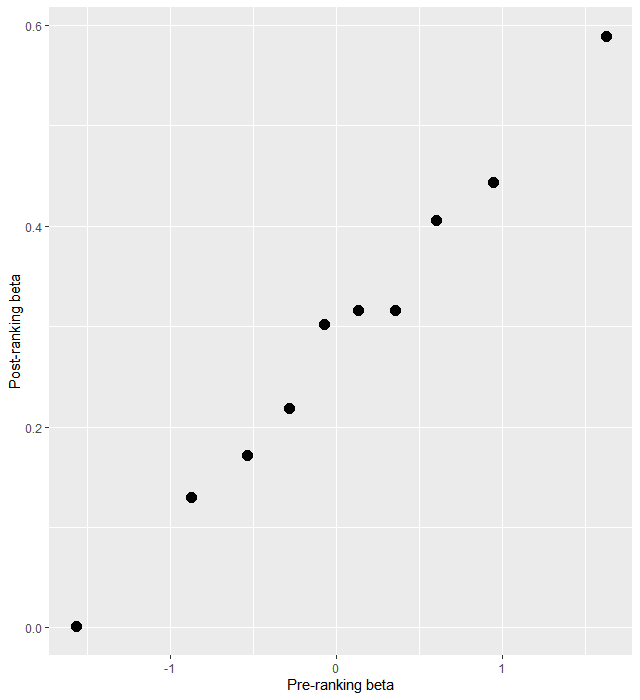
\includegraphics[width=0.60\textwidth]{paper_b3/Figure2.png}
\end{frame}


\scriptsize
\begin{frame}{Characteristics of decile portfolios, formed on $\beta_{CID}$}
\begin{table}[!htbp] \centering 
  \caption*{\textbf{Table 2: Characteristics of decile $\beta_{CID}$-sorted vw portfolios}} 
  \label{} 
\begin{tabular}{@{\extracolsep{-2pt}} lccccccccccc} 
\\[-1.8ex]\hline 
\hline \\[-1.8ex] 
 & D1 & D2 & D3 & D4 & D5 & D6 & D7 & D8 & D9 & D10 & LS \\ 
\hline \\[-1.8ex] 
Return & $1.16$ & $0.88$ & $0.85$ & $0.73$ & $0.63$ & $0.66$ & $0.66$ & $0.61$ & $0.54$ & $0.49$ & $$-$0.68$ \\ 
prebeta & $$-$1.57$ & $$-$0.87$ & $$-$0.54$ & $$-$0.29$ & $$-$0.07$ & $0.14$ & $0.35$ & $0.60$ & $0.95$ & $1.63$ & $3.20$ \\ 
postbeta & $0.002$ & $0.13$ & $0.17$ & $0.22$ & $0.30$ & $0.32$ & $0.32$ & $0.41$ & $0.44$ & $0.59$ & $0.60$ \\ 
size & $6.99$ & $7.58$ & $7.91$ & $8.19$ & $8.38$ & $8.61$ & $8.78$ & $8.92$ & $9.04$ & $8.88$ & $1.89$ \\ 
bm & $$-$0.83$ & $$-$0.76$ & $$-$0.76$ & $$-$0.73$ & $$-$0.73$ & $$-$0.74$ & $$-$0.74$ & $$-$0.77$ & $$-$0.83$ & $$-$0.86$ & $$-$0.03$ \\ 
op & $0.15$ & $0.16$ & $0.17$ & $0.17$ & $0.17$ & $0.17$ & $0.17$ & $0.17$ & $0.17$ & $0.17$ & $0.02$ \\ 
inv & $0.29$ & $0.22$ & $0.17$ & $0.16$ & $0.15$ & $0.13$ & $0.14$ & $0.14$ & $0.15$ & $0.17$ & $$-$0.12$ \\ 
$\beta$ & $1.02$ & $0.95$ & $0.92$ & $0.92$ & $0.92$ & $0.94$ & $0.96$ & $1.00$ & $1.07$ & $1.20$ & $0.18$ \\ 
BAspr & $0.41$ & $0.33$ & $0.27$ & $0.25$ & $0.23$ & $0.21$ & $0.19$ & $0.19$ & $0.18$ & $0.18$ & $$-$0.23$ \\ 
mom122 & $0.24$ & $0.17$ & $0.15$ & $0.13$ & $0.12$ & $0.12$ & $0.11$ & $0.11$ & $0.12$ & $0.13$ & $$-$0.11$ \\ 
vol1m & $2.40$ & $1.94$ & $1.77$ & $1.67$ & $1.62$ & $1.59$ & $1.58$ & $1.63$ & $1.71$ & $2.00$ & $$-$0.39$ \\ 
vol12m & $2.53$ & $2.04$ & $1.84$ & $1.75$ & $1.69$ & $1.67$ & $1.65$ & $1.71$ & $1.82$ & $2.16$ & $$-$0.38$ \\ 
$\beta_{VOL}$ & $$-$4.83$ & $$-$3.68$ & $$-$2.84$ & $$-$2.41$ & $$-$2.05$ & $$-$1.85$ & $$-$1.72$ & $$-$1.77$ & $$-$1.52$ & $$-$1.30$ & $3.53$ \\ 
$\beta_{CIV}$ & $$-$2.38$ & $$-$1.91$ & $$-$1.51$ & $$-$1.18$ & $$-$1.03$ & $$-$0.94$ & $$-$0.80$ & $$-$0.78$ & $$-$0.80$ & $$-$0.39$ & $1.99$ \\ 
\hline \\[-1.8ex] 
\end{tabular} 
\end{table}
\end{frame}



\begin{frame}{Returns of decile portfolios, formed on $\beta_{CID}$}
\begin{table}[!htbp] \centering 
  \caption*{\textbf{Table 3: Returns of decile $\beta_{CID}$-sorted portfolios}}
  \label{} 
\begin{tabular}{@{\extracolsep{-6pt}} cccccccccccc} 
\\[-1.8ex]\hline 
\hline \\[-1.8ex] 
 & D1 & D2 & D3 & D4 & D5 & D6 & D7 & D8 & D9 & D10 & LS \\ 
\hline \\[-1.8ex] 
Mean ew & 2.52 & 1.78 & 1.57 & 1.42 & 1.36 & 1.32 & 1.30 & 1.26 & 1.29 & 1.61 & -0.90$^{***}$ \\ 
T-stat ew & [9.94] & [8.88] & [8.31] & [7.96] & [7.62] & [7.46] & [7.09] & [6.65] & [6.52] & [6.61] & [-5.87] \\ 
Mean vw & 1.16 & 0.88 & 0.85 & 0.73 & 0.63 & 0.66 & 0.66 & 0.61 & 0.54 & 0.49 & -0.68$^{***}$ \\ 
T-stat vw & [4.87] & [4.52] & [4.64] & [4.15] & [3.82] & [4.04] & [3.89] & [3.61] & [2.98] & [2.24] & [-3.82] \\ 
\hline \\[-1.8ex] 
\end{tabular} 
\end{table}

% Table created by stargazer v.5.2.2 by Marek Hlavac, Harvard University. E-mail: hlavac at fas.harvard.edu
% Date and time: 10/14
\begin{table}[!htbp] \centering 
  \caption*{\textbf{Table 4: Abnormal returns of decile $\beta_{CID}$-sorted vw portfolios}} 
  \label{} 
\begin{tabular}{@{\extracolsep{0pt}} ccccccc} 
\\[-1.8ex]\hline 
\hline \\[-1.8ex] 
Statistic & Ret & $\alpha_{CAPM}$ & $\alpha_{FF3}$ & $\alpha_{Carhart}$ & $\alpha_{FF5}$ & $\alpha_{FF5+UMD+STR}$ \\ 
\hline \\[-1.8ex] 
LS & -0.68$^{***}$ & -0.65$^{***}$ & -0.74$^{***}$ & -0.53$^{***}$ & -0.79$^{***}$ & -0.48$^{***}$ \\ 
T-stat & [-3.82] & [-3.63] & [-4.45] & [-3.22] & [-4.62] & [-2.85] \\ 
\hline \\[-1.8ex] 
\end{tabular} 
\end{table}
\end{frame}



\begin{frame}{Factor loadings of decile portfolios, formed on $\beta_{CID}$}
\vspace{-0.25cm}
\begin{table}[!htbp] \centering 
  \label{} 
\begin{tabular}{@{\extracolsep{0pt}} ccccccccc} 
\\[-1.8ex]\hline 
\hline \\[-1.8ex] 
Ntile & Ret & Alpha & MKT & HML & SMB & RMW & CMA & adjR2 \\ 
\hline \\[-1.8ex] 
1 & 1.16 & 0.71 & 1.03 & -0.14 & 0.44 & -0.20 & -0.30 & 0.82 \\ 
 & [ 4.87] & [ 6.70] & [ 39.08] & [ -2.70] & [ 12.05] & [ -3.99] & [ -4.01] &  \\ 
2 & 0.88 & 0.34 & 0.97 & 0.00 & 0.24 & 0.09 & -0.12 & 0.83 \\ 
 & [ 4.52] & [ 3.95] & [ 46.02] & [ 0.06] & [ 8.29] & [ 2.17] & [ -2.05] &  \\ 
3 & 0.85 & 0.36 & 0.94 & -0.05 & 0.15 & 0.01 & -0.04 & 0.83 \\ 
 & [ 4.64] & [ 4.55] & [ 47.65] & [ -1.30] & [ 5.34] & [ 0.30] & [ -0.71] &  \\ 
4 & 0.73 & 0.15 & 0.96 & 0.00 & 0.10 & 0.15 & 0.06 & 0.86 \\ 
 & [ 4.15] & [ 2.23] & [ 55.99] & [ 0.06] & [ 4.12] & [ 4.44] & [ 1.29] &  \\ 
5 & 0.63 & 0.03 & 0.93 & 0.03 & 0.09 & 0.16 & 0.18 & 0.88 \\ 
 & [ 3.82] & [ 0.42] & [ 62.47] & [ 0.99] & [ 4.12] & [ 5.58] & [ 4.22] &  \\ 
6 & 0.66 & 0.11 & 0.93 & 0.02 & 0.00 & 0.14 & 0.11 & 0.88 \\ 
 & [ 4.04] & [ 1.82] & [ 63.52] & [ 0.66] & [ 0.01] & [ 4.84] & [ 2.61] &  \\ 
7 & 0.66 & 0.09 & 0.99 & 0.05 & -0.03 & 0.10 & 0.11 & 0.90 \\ 
 & [ 3.89] & [ 1.57] & [ 70.80] & [ 2.02] & [ -1.73] & [ 3.52] & [ 2.71] &  \\ 
8 & 0.61 & -0.01 & 1.01 & 0.15 & -0.08 & 0.18 & 0.10 & 0.91 \\ 
 & [ 3.61] & [ -0.22] & [ 76.79] & [ 5.83] & [ -4.19] & [ 7.00] & [ 2.59] &  \\ 
9 & 0.54 & -0.03 & 1.03 & 0.10 & -0.11 & 0.03 & 0.06 & 0.87 \\ 
 & [ 2.98] & [ -0.37] & [ 61.80] & [ 3.20] & [ -4.58] & [ 0.88] & [ 1.17] &  \\ 
10 & 0.49 & -0.08 & 1.15 & 0.19 & -0.05 & -0.15 & -0.14 & 0.82 \\ 
 & [ 2.24] & [ -0.80] & [ 48.49] & [ 4.05] & [ -1.60] & [ -3.16] & [ -2.05] &  \\ 
LS & -0.68 & -0.79 & 0.12 & 0.32 & -0.49 & 0.06 & 0.16 & 0.16 \\ 
 & [ -3.82] & [ -4.62] & [ 2.93] & [ 3.96] & [ -8.41] & [ 0.71] & [ 1.35] &  \\ 
\hline \\[-1.8ex] 
\end{tabular} 
\end{table}
\end{frame}



\begin{frame}{Fama-MacBeth}
\end{frame}



\begin{frame}{CID vs WID}
\begin{table}[!htbp] \centering 
  \caption*{\textbf{Table 8: Abnormal returns of 5x5 portfolios, double-sorted on within-industry dispersion $\beta_{WID}$ and $\beta_{CID}$}} 
  \label{} 
\begin{tabular}{@{\extracolsep{5pt}} ccccccc} 
\\[-1.8ex]\hline 
\hline \\[-1.8ex] 
Statistic & Ret & $\alpha_{CAPM}$ & $\alpha_{FF3}$ & $\alpha_{Carhart}$ & $\alpha_{FF5}$ & $\alpha_{FF5+UMD+STR}$ \\ 
\hline \\[-1.8ex] 
L/S WID & 0.16 & 0.25 & 0.13 & 0.00 & -0.12 & -0.16 \\ 
T-stat & [ 1.07] & [ 1.63] & [ 0.84] & [ 0.03] & [ -0.83] & [ -1.04] \\ 
L/S CID & 0.32$^{**}$ & 0.28$^{*}$ & 0.37$^{***}$ & 0.32$^{**}$ & 0.53$^{***}$ & 0.37$^{***}$ \\ 
T-stat & [ 2.32] & [ 1.92] & [ 2.68] & [ 2.25] & [ 3.81] & [ 2.60] \\ 
\hline \\[-1.8ex] 
\end{tabular} 
\end{table}
\end{frame}



\begin{frame}{CID and uncertainty measures}
\end{frame}



\begin{frame}{CID and CIV}
\end{frame}



\begin{frame}{CID and CIV: doublesorts}
\end{frame}



\begin{frame}{CID and CIV: Spanning tests}
\end{frame}



\begin{frame}{Other industry classifications}
\end{frame}



\begin{frame}{CID vs WID using FF5 industry classification}
\end{frame}



\begin{frame}{Economic channel: labor risk}
\end{frame}



\begin{frame}{Sectoral shifts hypothesis}
\end{frame}



\begin{frame}{Unemployment predictability}
\end{frame}



\begin{frame}{Future work}
\end{frame}



\begin{frame}{Conclusion}
\end{frame}



\begin{frame}{Appendix: $\beta_{CID}$ of FF49 industries}
\end{frame}



\begin{frame}{Appendix: Fama-MacBeth across stocks}
\end{frame}



\begin{frame}{Appendix: CID, constructed from abnormal industry returns}
\end{frame}



\begin{frame}{Appendix: CID vs CIV: Fama-MacBeth across $\beta_{CID}$-sorted portfolios}
\end{frame}



\begin{frame}{Appendix: CID vs CIV: Fama-MacBeth across $\beta_{CIV}$-sorted portfolios}
\end{frame}



\begin{frame}{2x3 Doublesort on $\beta_{CID}$ and size}
\end{frame}



\begin{frame}
\end{frame}



\begin{frame}
\end{frame}



\begin{frame}
\end{frame}



\begin{frame}
\end{frame}



\begin{frame}
\end{frame}



\begin{frame}
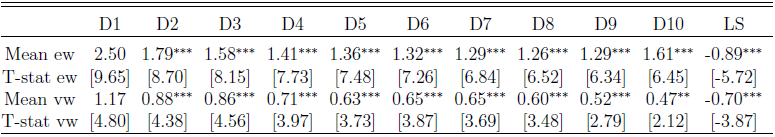
\includegraphics[width=1\textwidth]{table_spread.png}
\end{frame}




\end{document}

